\documentclass[12pt]{article}
\usepackage[a4paper]{geometry}
\geometry{verbose,tmargin=2cm,bmargin=2cm,lmargin=2cm,rmargin=2cm}
\usepackage{amsmath}
    
\setlength{\parindent}{0cm}
  
\usepackage{float}
\usepackage{graphicx}
\usepackage{enumitem}
\usepackage{hyperref}
\usepackage{url}
\usepackage{xcolor}

\usepackage{minted}
\newminted{scilab}{breaklines}

\definecolor{mintedbg}{rgb}{0.95,0.95,0.95}
\usepackage{mdframed}

\BeforeBeginEnvironment{minted}{\begin{mdframed}[backgroundcolor=mintedbg]}
\AfterEndEnvironment{minted}{\end{mdframed}}

\begin{document}

\title{Tugas Besar TF2202}
\date{}
\maketitle

\begin{scilabcode}
function [a,b] = func1(c,d)
  // Test comment
endfunction
\end{scilabcode}

Selesaikan soal-soal berikut ini dengan menggunakan Scilab.

%=====================================================
\section{Soal 1: Perbandingan akurasi beberapa metode}
%=====================================================

Carilah solusi numerik dari persamaan diferensial berikut
\begin{equation}
y'' + y = 0
\end{equation}
dengan syarat awal
\begin{equation}
y(0) = 0, \hspace{1cm} y'(0) = 1
\end{equation}

Bandingkan solusi yang diperoleh dengan solusi analitik:
\begin{equation}
y(t) = \sin(t)
\end{equation}

Gunakan menggunakan metode-metode berikut ini untuk mencari solusi numeriknya.
\begin{itemize}
\item Euler
\item Euler dengan prediktor-korektor (Runge-Kutta orde-2)
\item Runge-Kutta orde-4
\end{itemize}

Dari solusi numerik yang didapatkan, buatlah (1) plot antara $y$ dan $y'$
dan (2) plot antara $t$ dan $y$.

Bandingkan hasilnya pada interval $t$ dan parameter step ($h$) yang sama.

%=================================
\section{Soal 2: Gerakan pendulum}
%=================================

Gerak suatu pendulum dapat dinyatakan dengan persamaan diferensial:
\begin{equation}
u'' = -\frac{g}{L}\sin(u) - ku'
\end{equation}
dengan syarat awal
\begin{equation}
u(0) = u_0, \hspace{1cm} u'(t) = 0
\end{equation}
Dalam persamaan tersebut $u$ menyatakan simpangan pendulum,
$u_0$ menyatakan simpangan awal pendulum,
$g$ menyatakan percepatan gravitasi, $L$ menyatakan panjang benang pendulum,
dan $ku'$ menyatakan suku redaman (gesekan) yang berbanding lurus
dengan kecepatan $u'$ ($k$ adalah bilangan positif).

\begin{enumerate}[label=(\alph*)]
\item Cari solusi $u(t)$ untuk kasus $k=0$
\item Masih untuk kasus $k=0$, tentukan periode osilasi $T$ sebagai
fungsi dari simpangan awal $u_0$.
\item Carilah solusi $u(t)$ untuk kasus $k=0$
\end{enumerate}


%========================================================
\section{Soal 3: Persamaan Schrodinger (metode shooting)}
%========================================================

\begin{enumerate}[label=(\alph*)]
\item Persamaan Schrodinger independen-waktu pada 1 dimensi
dapat dinyatakan sebagai berikut.
\begin{equation}
-\frac{\hbar^2}{2m}\frac{\mathrm{d}\psi}{\mathrm{d}x^2}
+ V(x)\psi(x) = E\psi(x)
\label{eq:sch1d}
\end{equation}
Dengan menggunakan unit atomik, kita dapat mengambil $\hbar = 1$
dan $m = 1$, dan persamaan \eqref{eq:sch1d} dapat ditulis menjadi:
\begin{equation}
\psi'' = 2\left[ V(x) - E \right]\psi
\end{equation}

\item Metode shooting
\end{enumerate}

Metode shooting untuk quantum harmonic oscillator


%====================================================
\section{Soal 4: Persamaan Schrodinger (nilai eigen)}
%====================================================

(a) Finite difference orde h

(b) Finite difference orde h

%\textbf{SOLUSI}

Dengan menggunakan notasi berikut:
\begin{equation}
y_1 \equiv y, \hspace{1cm} y_2 \equiv y'
\end{equation}

%\begin{mdframed}[backgroundcolor=mintedbg]
%\inputminted[breaklines]{scilab}{soal_01.sce}
%\end{mdframed}


\begin{figure}[H]
\centering
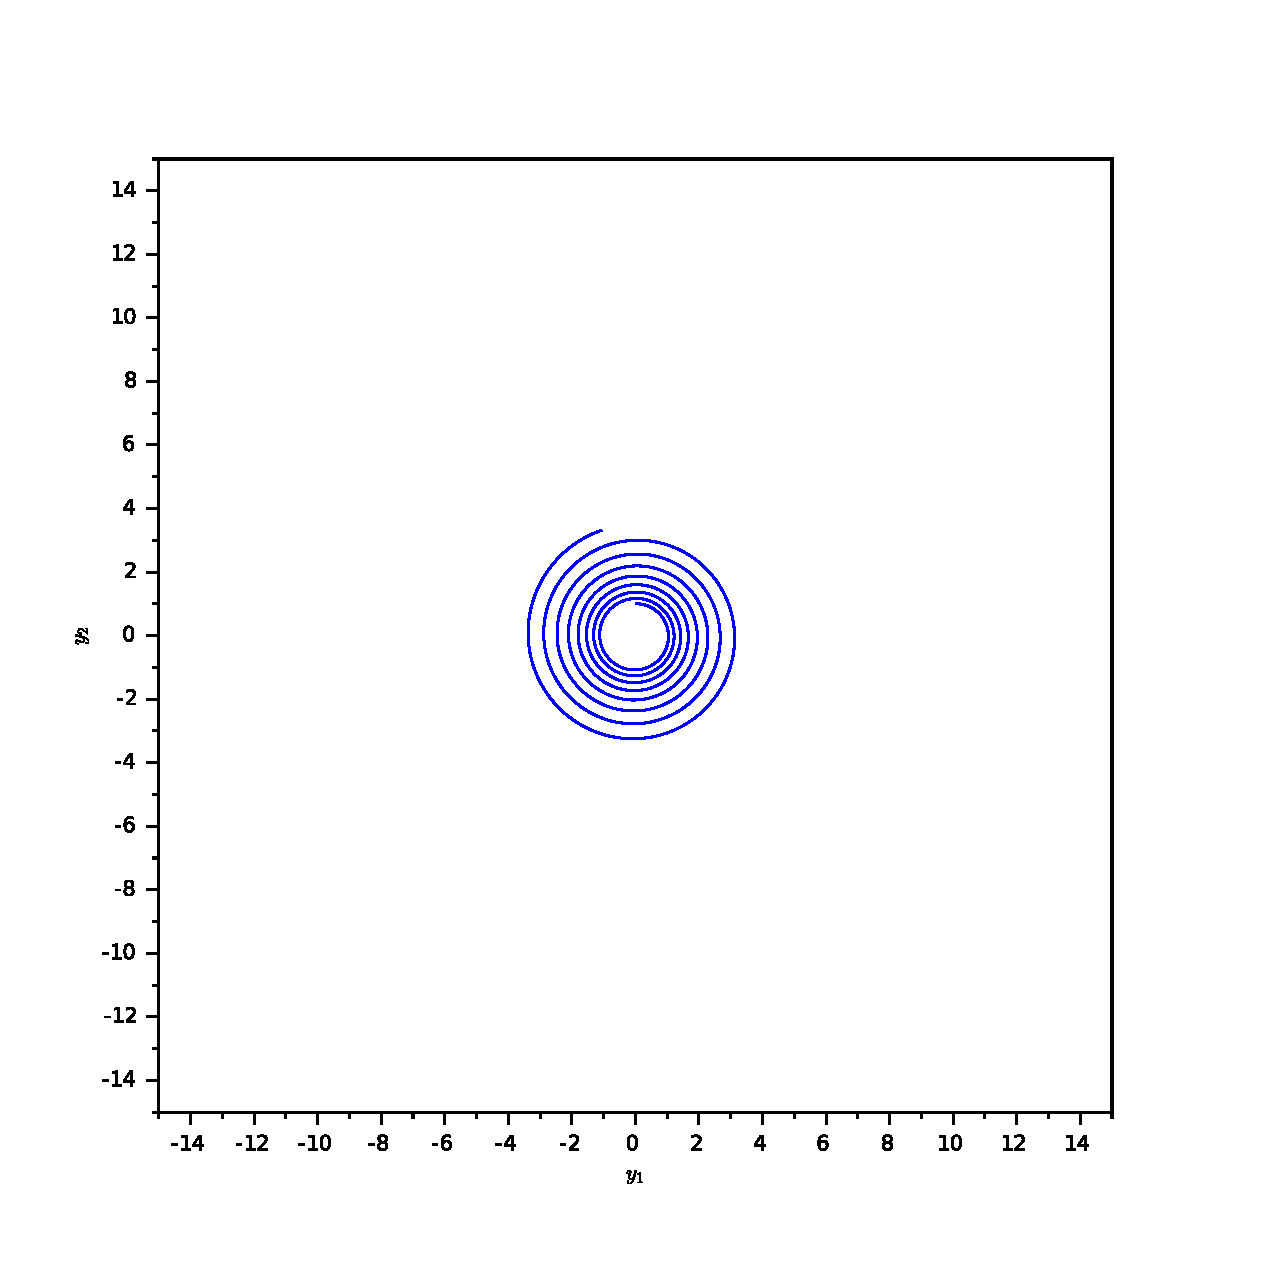
\includegraphics[width=0.3\textwidth]{images/soal_01_ode_euler_y1_y2.pdf}
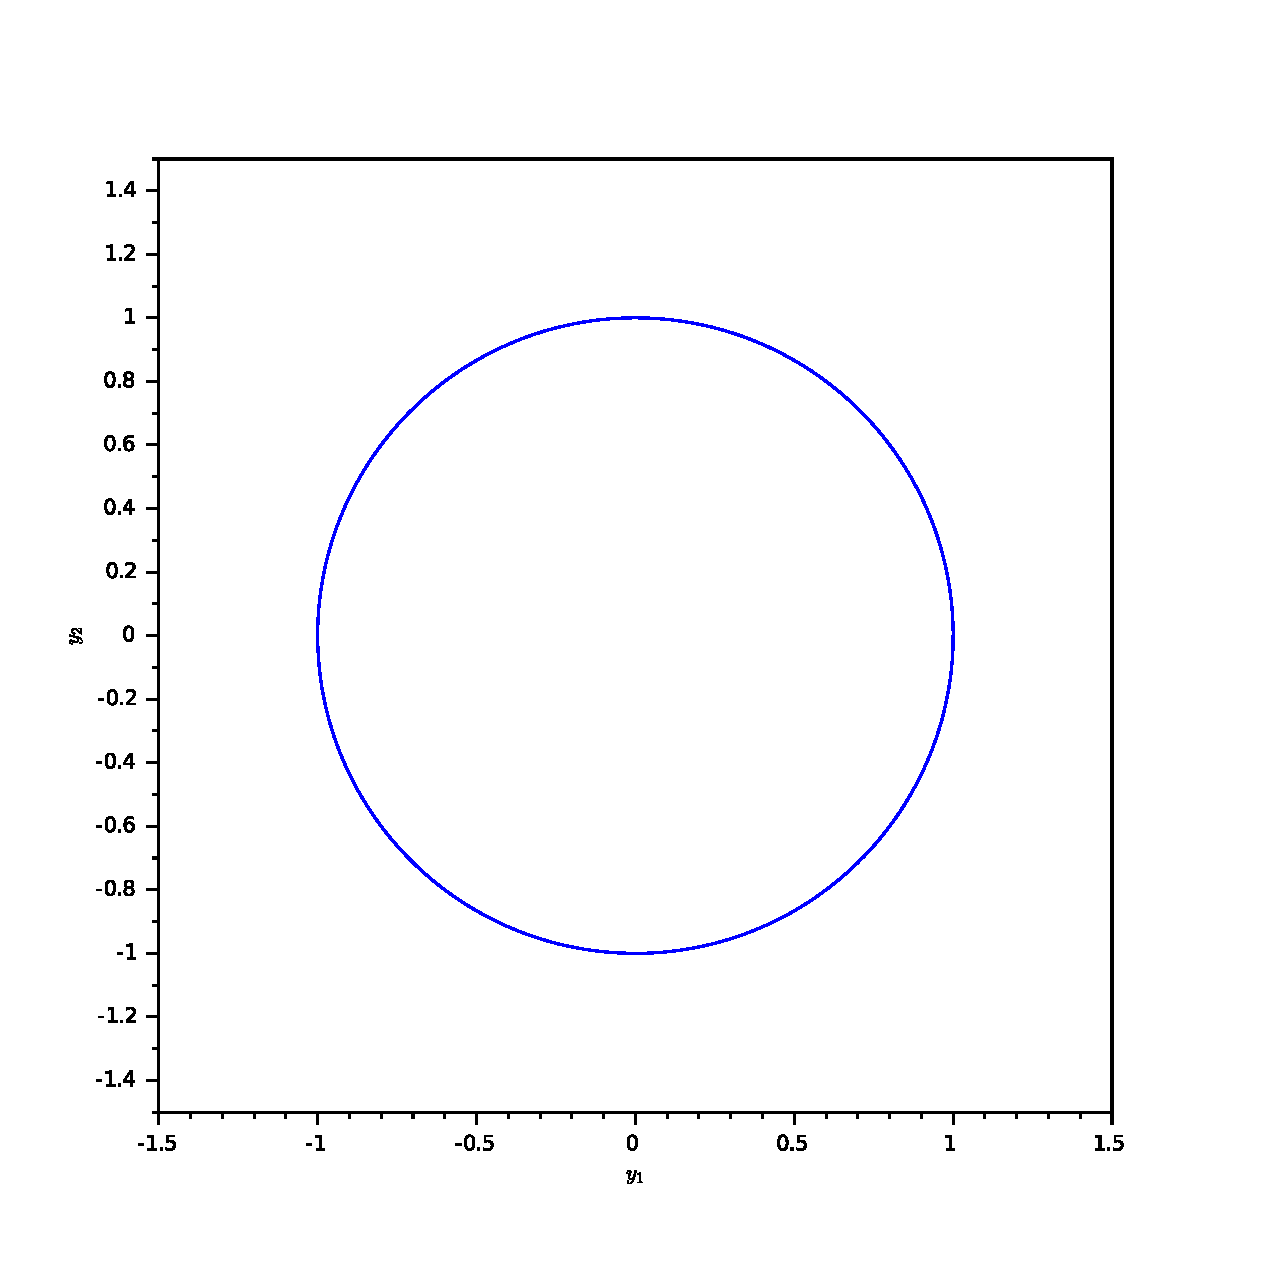
\includegraphics[width=0.3\textwidth]{images/soal_01_ode_euler_PC_y1_y2.pdf}
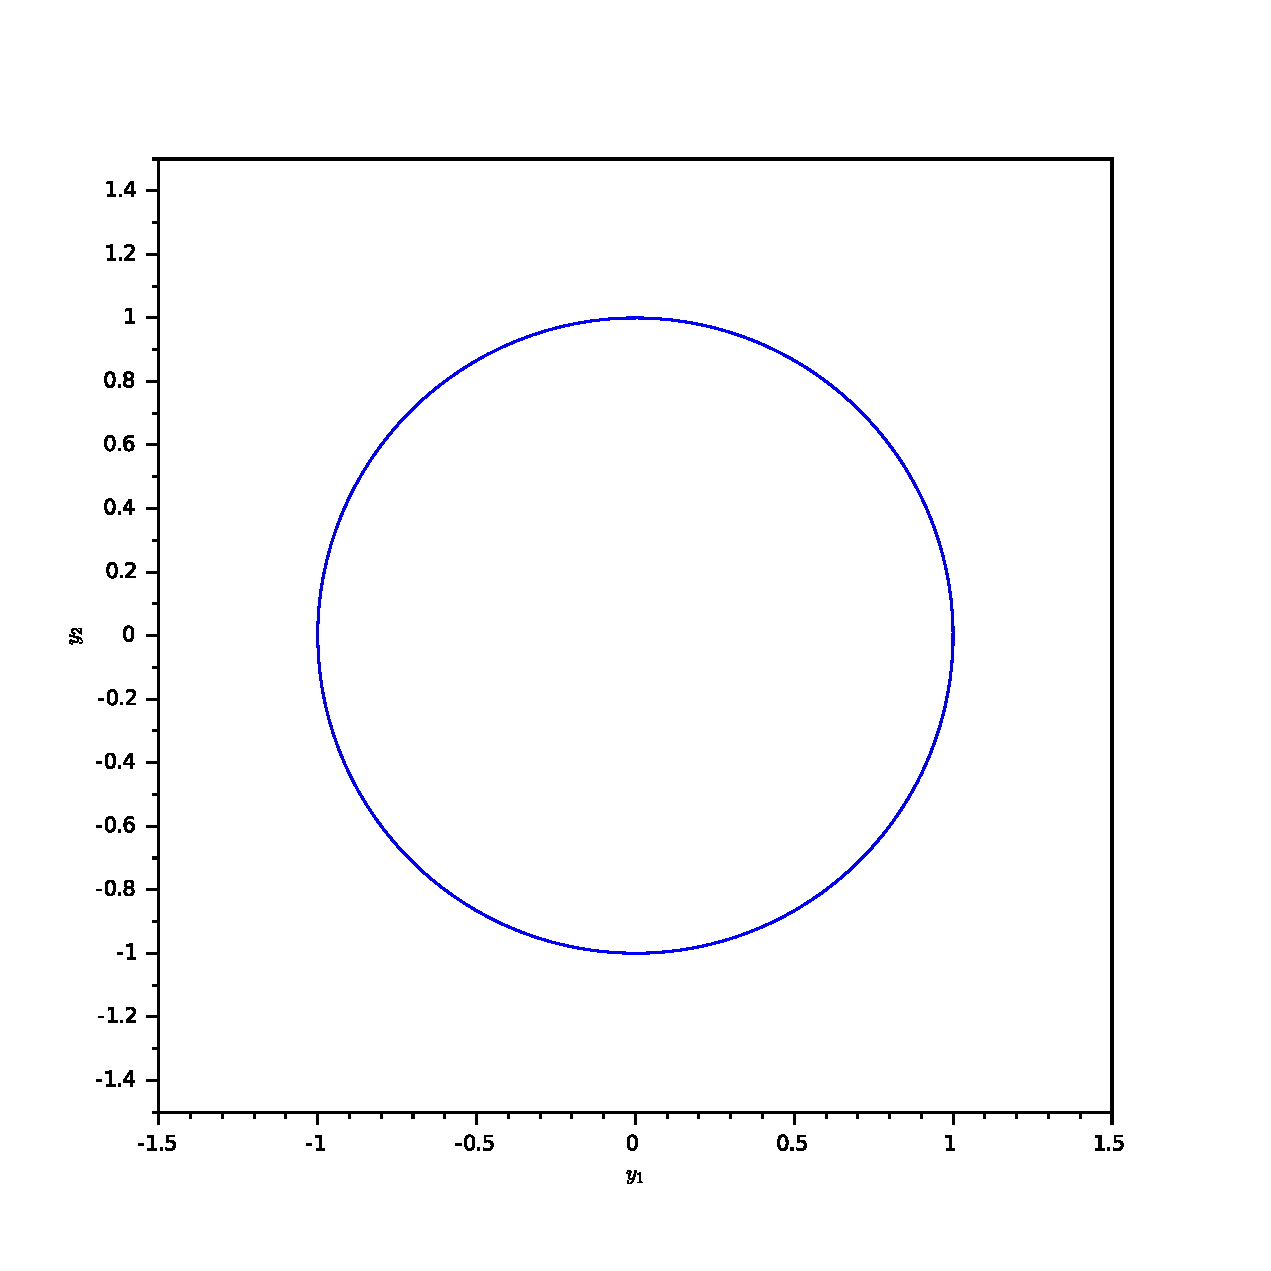
\includegraphics[width=0.3\textwidth]{images/soal_01_ode_RK4_y1_y2.pdf}
\par
\end{figure}

\begin{figure}[H]
\centering
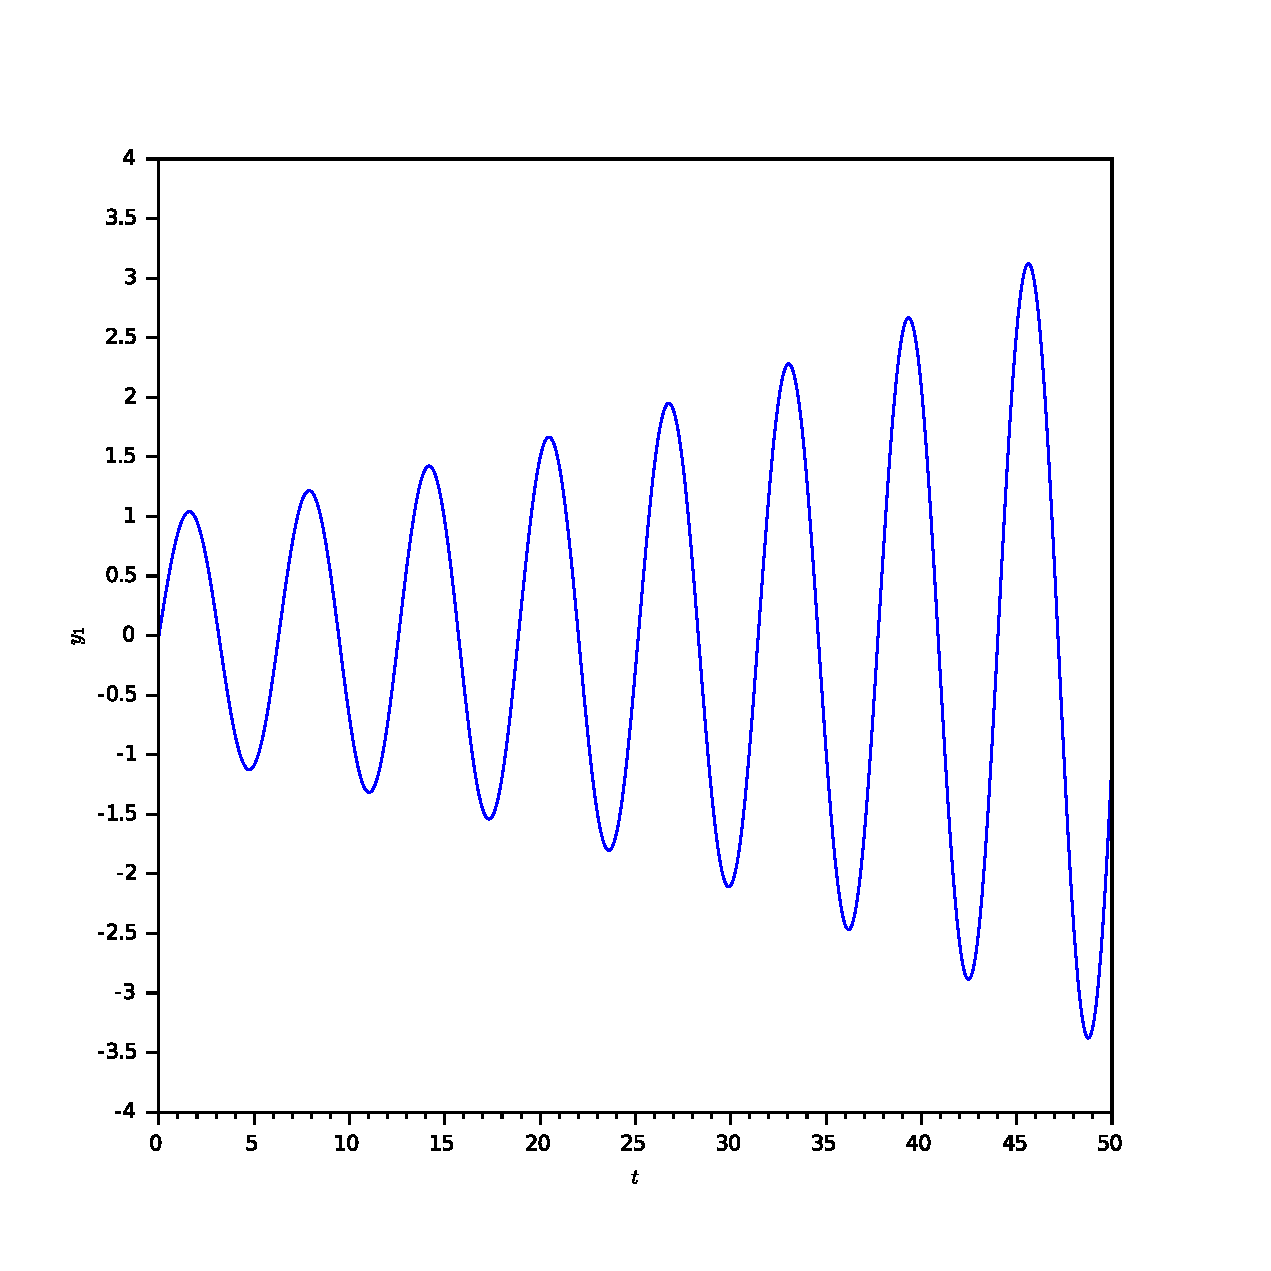
\includegraphics[width=0.3\textwidth]{images/soal_01_ode_euler_t_y1.pdf}
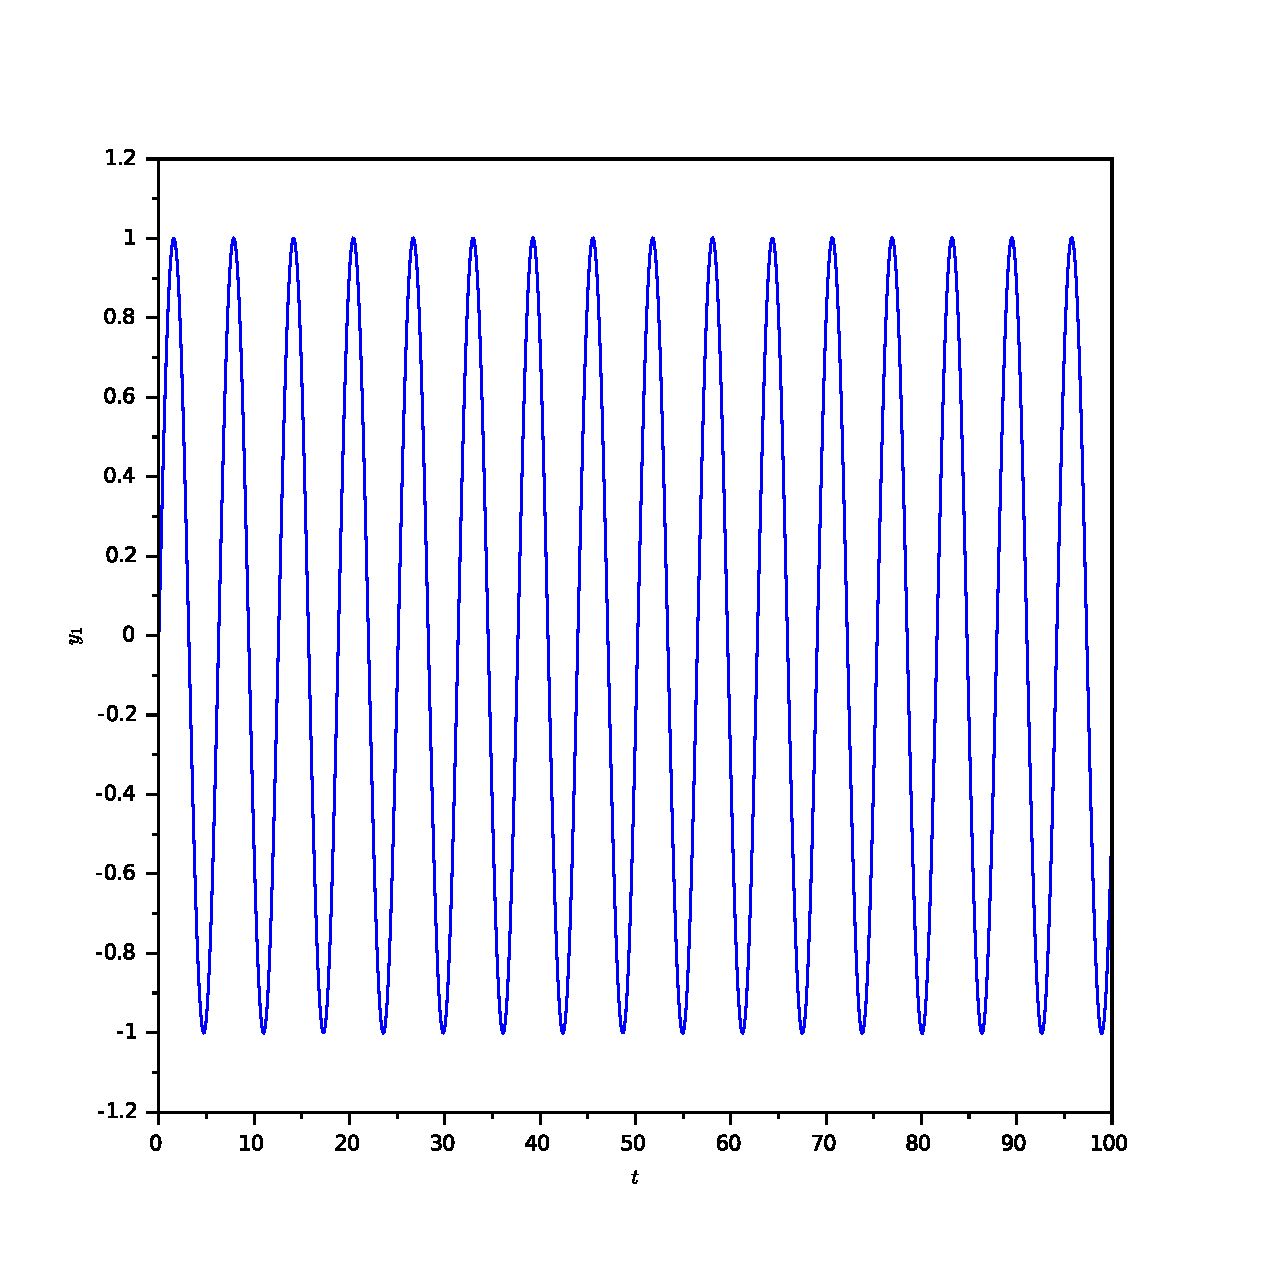
\includegraphics[width=0.3\textwidth]{images/soal_01_ode_euler_PC_t_y1.pdf}
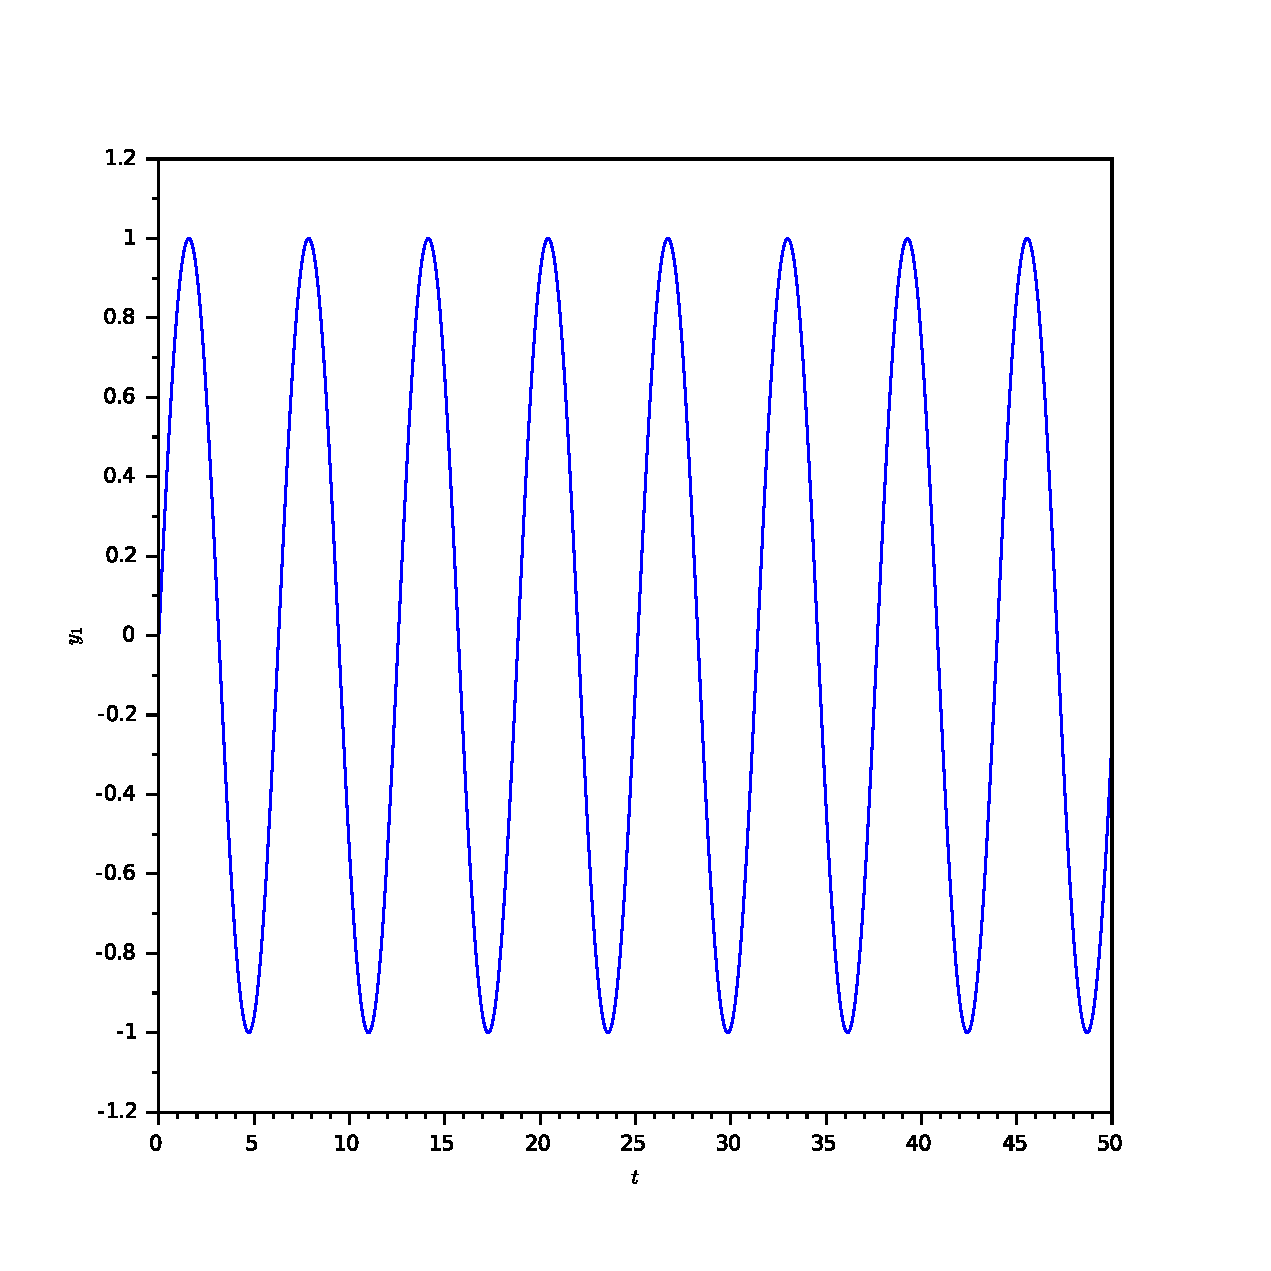
\includegraphics[width=0.3\textwidth]{images/soal_01_ode_RK4_t_y1.pdf}
\par
\end{figure}
%\section{Soal 2: Gerakan pendulum}

Gerakan pendulum
%\section{Soal 3: metode shooting}

soal a

soal b

Metode shooting untuk quantum harmonic oscillator

%\section{Soal 4: Persamaan Schrodinger melalui eigenvalue}

(a) harmonic oscillator
%\section{Soal 5: Persamaan Poisson 2D}
%\section{Soal 6: difusi dan kalor}
%\section{Soal 7: Persamaan gelombang}

\end{document}